%Use pdfLaTeX to compile

\documentclass[12pt,a4paper]{report}
\usepackage[pdftex]{graphicx}
\usepackage{titletoc} 
\usepackage{fancyhdr}   
\usepackage[a4paper,pdftex]{geometry}	
\usepackage[english]{babel}
\usepackage{xcolor} 
\usepackage{enumerate}
\usepackage{fix-cm} 
\usepackage[notlof]{tocbibind}
\usepackage{amsmath}
\usepackage{listings}

\bibliographystyle{ieeetr}  
\usepackage[toc,page]{appendix}

\begin{document}
\begin{titlepage}
\begin{center}

\includegraphics[scale=1.5]{CoverSheet}\\
\bf{ DEPARTMENT OF ELECTRICAL AND ELECTRONIC ENGINEERING }
\end{center}

\vspace{18mm}
 \begin{center}
 \begin{Large}
 {EEE212 Project Report}\\ 
 \vspace{2.0cm}
 \bf{Smart Refrigerator}
 \end{Large}
 \end{center} 
\vspace{2.0cm}

  \begin{center}
  \begin{large}
   \vspace{3.0cm}
     \begin{tabular}{r@{ }l} 
       Student Name : & Your Name\\ 
       Student ID : & Your student ID\\ 
       Supervisor : &  Your supervisor's name\\ 
       Assessor : & Your accessor's name \\
    \end{tabular}
  \end{large}
  \end{center}
\clearpage
\end{titlepage}

\abstract{Write your abstract here}

\tableofcontents


\quad 
\setcounter{page}{1}
\chapter{Introduction}
Home appliances have become a necessary part of our lives, providing comfort and luxury. A refrigerator is one such appliance that is crucial in one's household, rarely powered off. It is an engineering feat, which combines multiple engineering fields under one. The hardware and electronics are in perfect sync with each other providing cooling. This is the main reason that we chose to build a mini-refrigerator for this project. Our aim was to build a small fridge, one that could cool 3-4 cans of drinks. It would require no manual temperature control, i.e. the cooling inside the fridge was automatically controlled when the temperature dropped too low and vice versa. The report that follows describes how the project was approached, progressed and finally completed, with results and observations explained. It would attempt to become a guide to those who would want to build this mini-fridge. 

\chapter{Background}
\section{Peltier Effect}
The Peltier effect can be described as the temperature difference created when voltage is applied between two pieces of electrodes or conductor, which are directly connected to a a semiconductor. It is also called the Thermoelectric effect, as a thermoelectric device is used to create a voltage difference in most cases. The Peltier effect allows heat or cold to be transferred from one medium to the other, utilizing the current flow between the two conductors. The figure below illustrates the Seebeck Circuit, which is used in cooling applications such as in a refrigerator. 

\begin{figure}[!h]
	\centering
	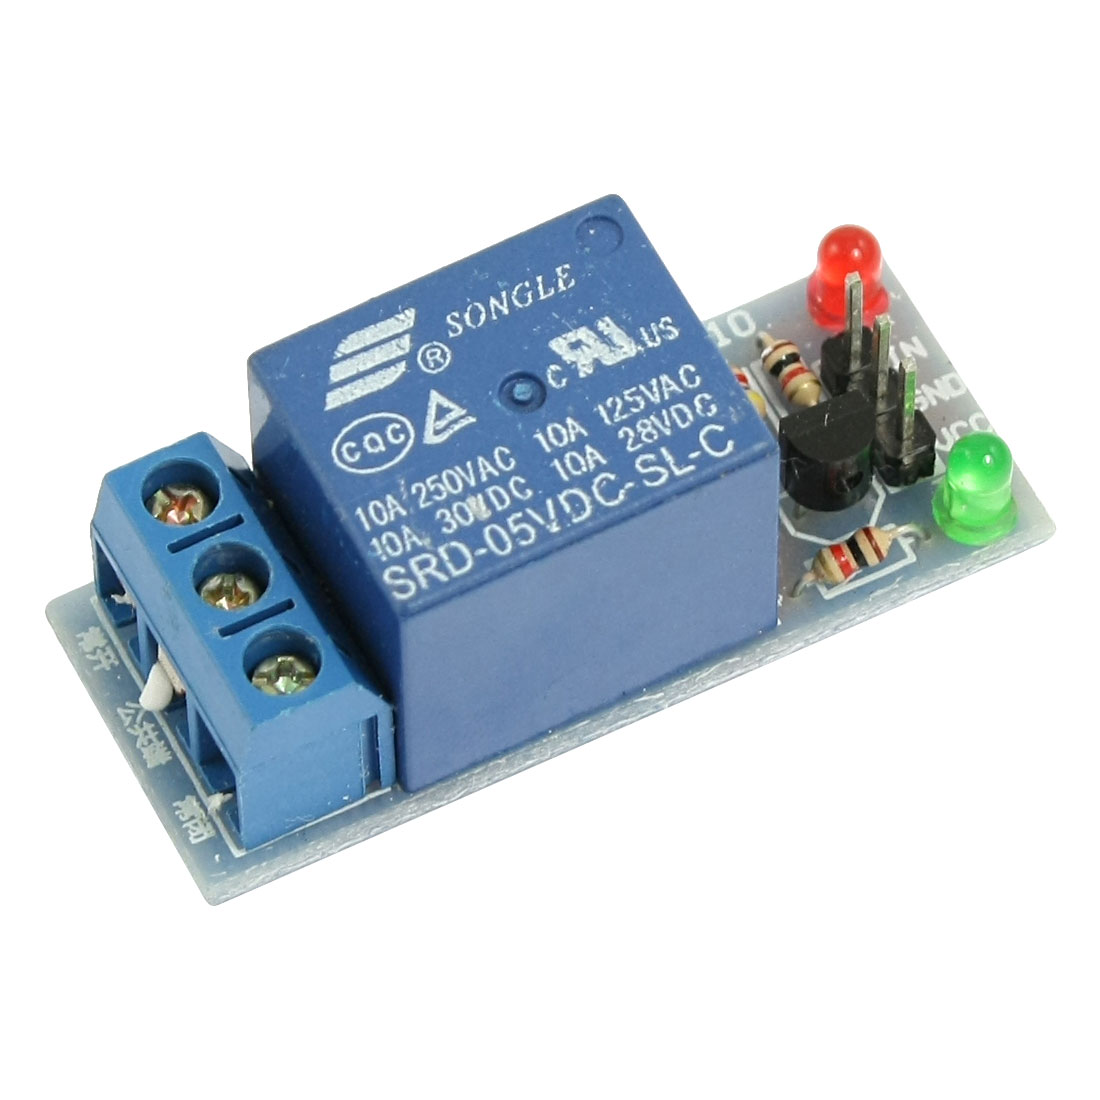
\includegraphics[scale=0.1]{relay}
	\caption{Magnetic Latching Relay}
\end{figure}

\section{Relay}
A relay is an electrically operated switch. Many switch on/off
mechanically using electromagnets.\\
Relays are used where it is necessary to control a circuit by a specific
low-power signal. For our project, we used a Magnetic Latching Relay
with a single coil. The relay operates in one direction when power is
applied with one polarity, and will reset when polarity is reversed
\begin{figure}[!h]
	\centering
	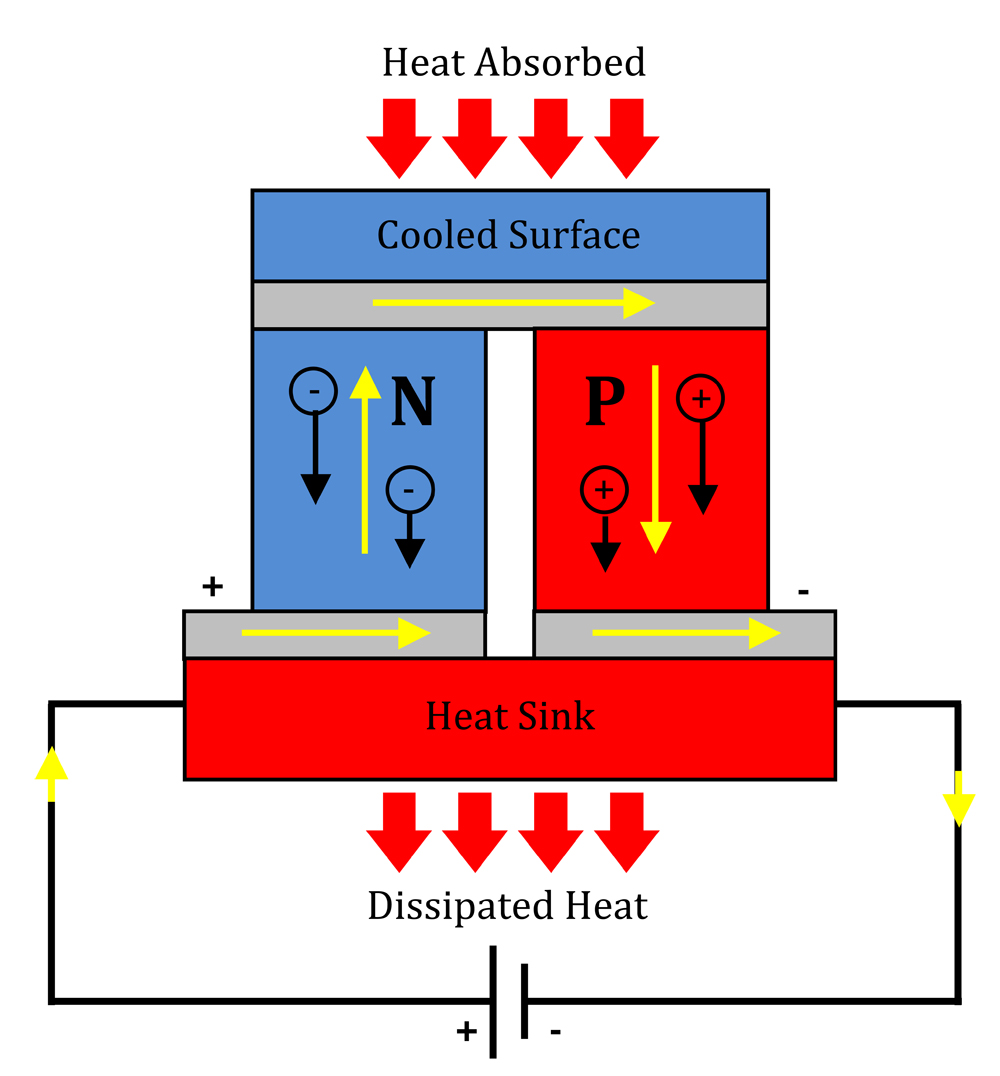
\includegraphics[scale=1.4]{peltier_effect}
	\caption{The Seebeck circuit as the peltier cooler}
\end{figure}



\chapter{Methodology} 
Describe your method here: the Asymptote and Matlab programming languages that you use in this project.

\section{Item List}
Following is the equipment used in building the refrigerator:
\begin{itemize}\itemsep -2pt
\item 12V 6A Thermoelectric Cooler
\item Magnetic Latching Relay module
\item Arduino Nano
\item Temperature Sensor
\item 12V 10A power supply
\item Perforated Board
\item Soldering Equipment
\item Foam boards
\item Hinges
\item Plexiglass Panels
\item Hot Glue-gun
\item Pro's Kit Mini-drill
\end{itemize}

\section{Circuit Schematic}
\begin{figure}[!h]
	\centering
	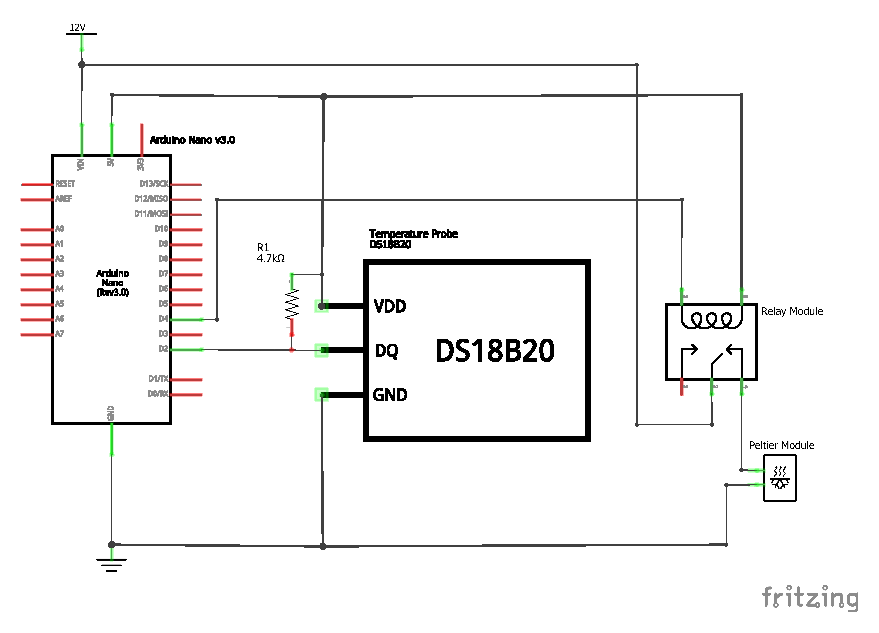
\includegraphics[scale=1.0]{mini_fridge_schem}
	\caption{Circuit Schematic of our control circuit}
\end{figure}
********Explain here*****


\section{Procedure}
The following procedure was followed when assembling the refrigerator. 
\begin{itemize}\itemsep -2pt
	\item In order to build the refrigerator, plexiglass panels were used. The reason being because they are cheaper than other materials and temperature insensitive. The panels were cut to dimensions and assembled using hot-glue gun. The whole box was split into 2 compartments, back one for the all the electronic equipment, while the front compartment would act as the fridge.
	\item Foam boards were glued to the inside of the refrigerator when box was completed. This would lated provide insulation from the heat outside, trapping the cool air in. 
	\item The thermoelectric cooler was then placed in between the back and the front compartment. 
	\item The Arduino circuit was then assembled using the circuit schematic explained previously. 
	\item After testing the circuit was functional, the doors were attached to the fridge in the front. The back compartment was kept open, exposed to air, in order maintain air flow. The hot air from the cooler was able to escape easily. 
	\item After fully assembled, multiple tests were conducted in order to test the temperature and cooling inside the fridge. These are discussed in the next chapter. 
\end{itemize}

\chapter{Result and Discussion}
The section below discusses our results and observations for the mini-fridge. 

\section{Figure}
 ***picture of our final product***

 






\chapter{Improvement}
Describe the improvements that you have done in this project.

\chapter{Conclusion}
Here comes the conclusion!

%\begin{thebibliography}{x}
%%\bibitem{avinash11pc} Avinash (2011, Dec.25). PC Controlled Robot [Online]. Available: http://extremeelectronics.co.in/avr-projects/pc-controlled-robot/
%
%\bibitem{wendlandt05indoor} Wendlandt, K.; Berhig, M.; Robertson, P., "Indoor localization with probability density functions based on Bluetooth," Personal, Indoor and Mobile Radio Communications, 2005. PIMRC 2005. IEEE 16th International Symposium on, vol.3, no., pp.2040,2044 Vol. 3, 11-14 Sept. 2005
%
%\end{thebibliography}


\bibliographystyle{IEEEtran}
\bibliography{ref}

\begin{appendices}
\begin{verbatim}
The whole codes:

#include<IRremote.h>
#include<Wire.h>
#include <LiquidCrystal_I2C.h>
LiquidCrystal_I2C lcd(0x27, 16, 2);



int RECV_PIN = 11; 
IRrecv irrecv(RECV_PIN); 
decode_results results; 

int AIN1 = 6; //PWMA
int AIN2 = 5; //DIRA
int BIN1 = 10; //PWMB
int BIN2 = 9; //DIRB
int sensorPin = A0; 
int ledPin = 13; 
int sensorValue = 0; 



int melody[] = {330, 330, 330, 262, 392, 200, 280};
int noteDurations[] = {8, 4, 4, 8, 4, 4, 6};

void setup() 
{
pinMode(AIN1, OUTPUT);
pinMode(AIN2, OUTPUT);
pinMode(BIN1, OUTPUT);
pinMode(BIN2, OUTPUT);
pinMode(ledPin, OUTPUT);
Serial.begin(9600);


}
}
\end{verbatim}

%Example of Matlab code, remember to include "listings" package
\begin{lstlisting}[language={MATLAB}, keywordstyle=\color{blue!70},commentstyle=\color{green!40!black},frame=shadowbox, rulesepcolor=\color{red!20!green!20!blue!20},basicstyle=\footnotesize]
%Justification via Matlab of function 36%
clc;clear;
syms x y Fx Fy A B C D;
z=100*(x-y^2)^2+(1-x)^2+10.1*(y-1)^2
Fx=diff(z,x)
Fy=diff(z,y)
S=solve(Fx,Fy);
x1=S.x
y1=S.y
A=diff(z,x,2)
B=diff(diff(z,x),y)
C=diff(z,y,2)
D=A*C-B^2
D1=subs(subs(D,'x',x1(1)),'y',y1(1))
A1=subs(subs(A,'x',x1(1)),'y',y1(1))
Z1=subs(subs(z,'x',x1(1)),'y',y1(1))
\end{lstlisting}

\end{appendices}
\end{document}
